\section{پردازشگر‌های زبان}
\begin{frame}[fragile]{پردازش‌گر‌های زبان}
\begin{itemize}\itemr
\item[-]
به بیان ساده، کامپایلر برنامه‌ایست که می‌تواند یک برنامه را با یک زبان (\lr{\textit{source} language}) بخواند، و معادل آن را به زبانی دیگر ترجمه کند  (\lr{\textit{targer} language}.)
\vspace{5mm}
\begin{figure}[H]
\begin{center}
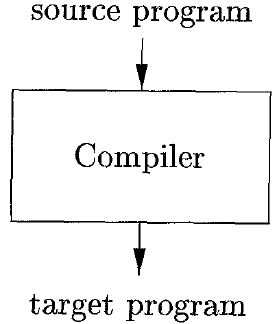
\includegraphics[width=0.3\textwidth, height=0.6\textheight, angle=1]{docs/images/sct}
\end{center}
\end{figure}
\end{itemize}
\end{frame}

\begin{frame}{برنامه‌ی ترجمه شده}
\begin{itemize}\itemr
\item[-]
اگر برنامه‌ی تولید شده، یک 
\lr{executable machine-language program}
باشد، می‌توان آن را مستقیما توسط پردازنده اجرا کرد.
\vspace{5mm}
\begin{figure}[H]
\begin{center}
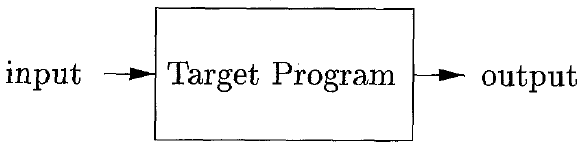
\includegraphics[width=0.6\textwidth, height=0.3\textheight, angle=0.5]{docs/images/executable}
\end{center}
\end{figure}
\end{itemize}
\end{frame}

\begin{frame}{مفسر}
\begin{itemize}\itemr
\item[-]
نوع دیگری از پردازش‌گر‌های زبانی، مفسرها هستند که بجای تبدیل زبان به زبان دیگر (\lr{\textit{target}})، خود مستقیما مسئول اجرای زبان اول (\lr{\textit{source}}) می‌شوند.
\vspace{5mm}
\begin{figure}[H]
\begin{center}
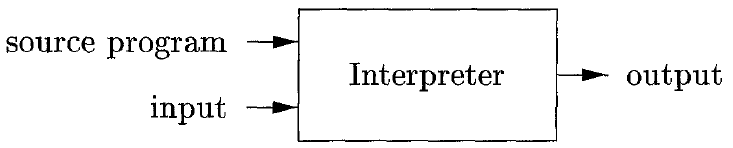
\includegraphics[width=0.7\textwidth, height=0.3\textheight, angle=0]{docs/images/interpreter}
\end{center}
\end{figure}
\end{itemize}
\end{frame}
